\section{Kontrollstrukturen}
	\begin{minipage}[t]{9 cm}
		\subsection{Sequenz \verweis{8.1}}
			Die Sequenz ist eine zeitlich geordnete Abfolge von Anweisungen. \\
				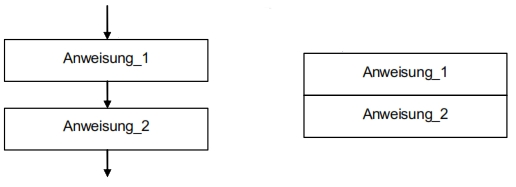
\includegraphics[width=1\textwidth]{pics/Sequenz.jpg}	
			
	\end{minipage}
	%
	\begin{minipage}[t]{9 cm}
			\subsubsection{Block}
				\begin{compactitem}
					\item Erfordert die Syntax genau eine Anweisung, so können dennoch mehrere Anweisungen geschrieben werden, wenn man sie in Form eines Blocks zusammenfasst.
					\item Ein Block wird mit geschweiften Klammern eingefasst. $\{ \dots \}$ Ein Block zählt syntaktisch als eine einzige Anweisung.
				\end{compactitem}
				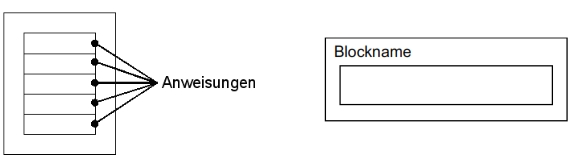
\includegraphics[width=1\textwidth]{pics/Block.jpg}
	\end{minipage}	
		
	\subsection{Selektion \verweis{8.2}}
		Von \textbf{Selektion} spricht man zum einen, wenn man eine Anweisung nur dann ausführen will, wenn eine bestimmte Bedingung zutrifft. Zum anderen möchte man mit Selektionsanweisungen zwischen zwei Möglichkeiten (entweder/oder) bzw. zwischen mehreren Möglichkeiten genau eine auswählen.\\
		
		\begin{minipage}[t]{5.5 cm}
			\subsubsection{Einfache Alternative}
				\lstinputlisting[language=C,tabsize=2]{code/strukturen_if_else.c}
		\end{minipage}
		%
		\begin{minipage}[t]{5.5 cm}
			\subsubsection{Bedingte Anweisung}
				\lstinputlisting[language=C,tabsize=2]{code/strukturen_if.c}
		\end{minipage}
		%
		\begin{minipage}[t]{7 cm}
			\subsubsection{Mehrfache Alternative - else if}
				\lstinputlisting[language=C,tabsize=2]{code/strukturen_else_if.c}
		\end{minipage}
		
%%%%%%%%%%%%%%%%%%%%%%%%%%%%%%%%%%%%%%%%%%%%%%%%%%%%%%%%%%%%%%%%%%%%%%%%%%%%%%%%%%%%%%%%%%%%%%%%%%%%%%%%%	
\newpage%%%%%%%%%%%%%%%%%%%%%%%%%%%%%%%%%%%%%%%%%%%%%%%%%%%%%%%%%%%%%%%%%%%%%%%%%%%%%%%%%%%%%%%%%%%%%%%%%
%%%%%%%%%%%%%%%%%%%%%%%%%%%%%%%%%%%%%%%%%%%%%%%%%%%%%%%%%%%%%%%%%%%%%%%%%%%%%%%%%%%%%%%%%%%%%%%%%%%%%%%%%
	
		\subsubsection{Mehrfache Alternative - switch case}
			\begin{minipage}[t]{9 cm}
				
				\begin{compactitem}
					\item Für eine Mehrfach-Selektion, d.h. eine Selektion unter mehreren Alternativen, kann die $switch$-Anweisung verwendet werden, falls die Alternativen ganzzahligen Werten eines Ausdrucks von einem Integer-Typ entsprechen.
					\item Hat der Ausdruck der $switch$-Anweisung den gleichen Wert wie einer der konstanten Ausdrücke der $case$-Marken, wird die Ausführung des Programms mit der Anweisung hinter dieser $case$-Marke weitergeführt.
					\item Stimmt keiner der konstanten Ausdrücke mit dem $switch$-Ausdruck überein, wird zu $default$ gesprungen.
				\end{compactitem}							
			\end{minipage}
			\hspace*{1cm}
			\begin{minipage}[t]{9 cm}
				\vspace*{-0.5cm}
				\lstinputlisting[language=C,tabsize=2]{code/strukturen_switch.c}
			\end{minipage}
		
	\subsection{Iteration \verweis{8.3}}
		\begin{minipage}[t]{4 cm}
			\subsubsection{While}
				\lstinputlisting[language=C,tabsize=2]{code/strukturen_while.c}
		\end{minipage}
		%
		\begin{minipage}[t]{10 cm}
			\subsubsection{For-Schleife}
				\lstinputlisting[language=C,tabsize=2]{code/strukturen_for.c}
		\end{minipage}
		%
		\begin{minipage}[t]{5 cm}
			\subsubsection{Do-While}
				\lstinputlisting[language=C,tabsize=2]{code/strukturen_dowhile.c}
		\end{minipage}
		
		\subsubsection{Endlosschleife}
			\begin{minipage}[c]{3 cm}
				\lstinputlisting[language=C,tabsize=2]{code/strukturen_endlos_for.c}
			\end{minipage}
			%
			\begin{minipage}[c]{3 cm}
				\lstinputlisting[language=C,tabsize=2]{code/strukturen_endlos_while.c}
			\end{minipage}
		
		\subsubsection{Wann wird welche Schleife eingesetzt?}
			\begin{compactitem}
				\item For-Schleife: Bei Zählschleifen, d.h. wenn die Anzahl Durchläufe (kann auch variabel sein) im
				voraus feststeht.
				\item Do-While-Schleife: Wenn es keine Zählschleife ist, und die Schleife muss mindestens einmal
				durchlaufen werden
				\item While-Schleife: In allen anderen Fällen
			\end{compactitem}
			
	\subsection{Sprunganweisungen \verweis{8.4}}
		\begin{compactitem}
			\item $break$: $do-while$-, $while$-,  $for$-Schleife und $switch$-Anweisung abbrechen
			\item $continue$: in den nächsten Schleifendurchgang (Schleifenkopf) springen bei $do-while$-, $while$- und $for$-Schleife 
			\item $return$: aus Funktion an aufrufende Stelle zurückspringen
			\item $goto$: innerhalb einer Funktion an eine Marke (Label) springen
		\end{compactitem}